%%%%%%%%%%%%%%%%%%%%%%%%%%%%%%%%%%%%%%%%%%%%%%%%%%%%%%%%%%%%%%%%%%%%%%%%%%%%%%
%
% Section file included in main project file using \input{}
%
% Assumes that LaTeX2e macros and packages defined in cg_comp.sty are
%   available
%
%%%%%%%%%%%%%%%%%%%%%%%%%%%%%%%%%%%%%%%%%%%%%%%%%%%%%%%%%%%%%%%%%%%%%%%%%%%%%%

 \section{Simple Model of Guitar Intonation\label{sct:model}}
The starting point for prior efforts to understand guitar intonation and compensation~\cite{ref:byers1996cgi,ref:varieschi2010icf} is a formula for $f_{m}$, the transverse vibration frequency harmonic $m$ of a stiff string, originally published by Morse in 1936~\cite{ref:morse1981vsb}:
 \begin{equation}\label{eqn:f_m_clamped}
f_{m} = \frac{m}{2\, L}\, \sqrt{\frac{T}{\mu}} \left[ 1 + 2 B + 4 \left(1 + \frac{\pi^2\, m^2}{8}\right) B^2 \right]\, .
 \end{equation}
Here $L$ is the length of the string, $T$ and $\mu$ are its tension and the linear mass density, respectively, and $B$ is a small ``bending stiffness'' coefficient to capture the relevant mechanical properties of the string. For a homogeneous string with a cylindrical cross section, $B$ is given by
 \begin{equation} \label{eqn:b_def}
B \equiv \sqrt{\frac{\pi\, \rho^4\, E}{4\, T\, L^2}}\, ,
 \end{equation}
where $\rho$ is the radius of the string and $E$ is Young's modulus (or the modulus of elasticity). But it's unlikely that \eqn{f_m_clamped} accurately describes the resonant frequencies of a nylon string on a classical guitar, because it assumes that the string is ``clamped'' at both ends, so that a particular set of symmetric boundary conditions must be applied to the partial differential equation (PDE) describing transverse vibrations of the string. We believe that this assumption is correct for the end of the string held at either the nut or the fret, but that the string is ``pinned'' (and not clamped) at the saddle. In \app{freq}, we solve the PDE using these non-symmetric boundary conditions, and find
 \begin{equation} \label{eqn:f_m_stiff}
f_m = \frac{m}{2\, L}\, \sqrt{\frac{T}{\mu}} \left[ 1 + B + \left( 1 + \half m^2 \pi^2 \right) B^2 \right]\, .
 \end{equation}
Note that this expression is valid only when $B \ll 1$. For a typical nylon guitar string with $E \approx 5$~GPa, $T \approx 60$~N, $\rho \approx 0.5$~mm, and $L \approx 650$~mm, we have $B \approx 3 \times 10^{-3}$. (In this case, the quadratic term in $B$ is only 2\% as large as the linear term, and can generally be neglected. We will include it in our analysis below only for completeness.) We'll use \eqn{f_m_stiff} with some caution, because the physics of nylon strings (particularly the wound base strings) are quite complicated~\cite{ref:lynchaird2017mpn}.

 \begin{figure}
  \centering
  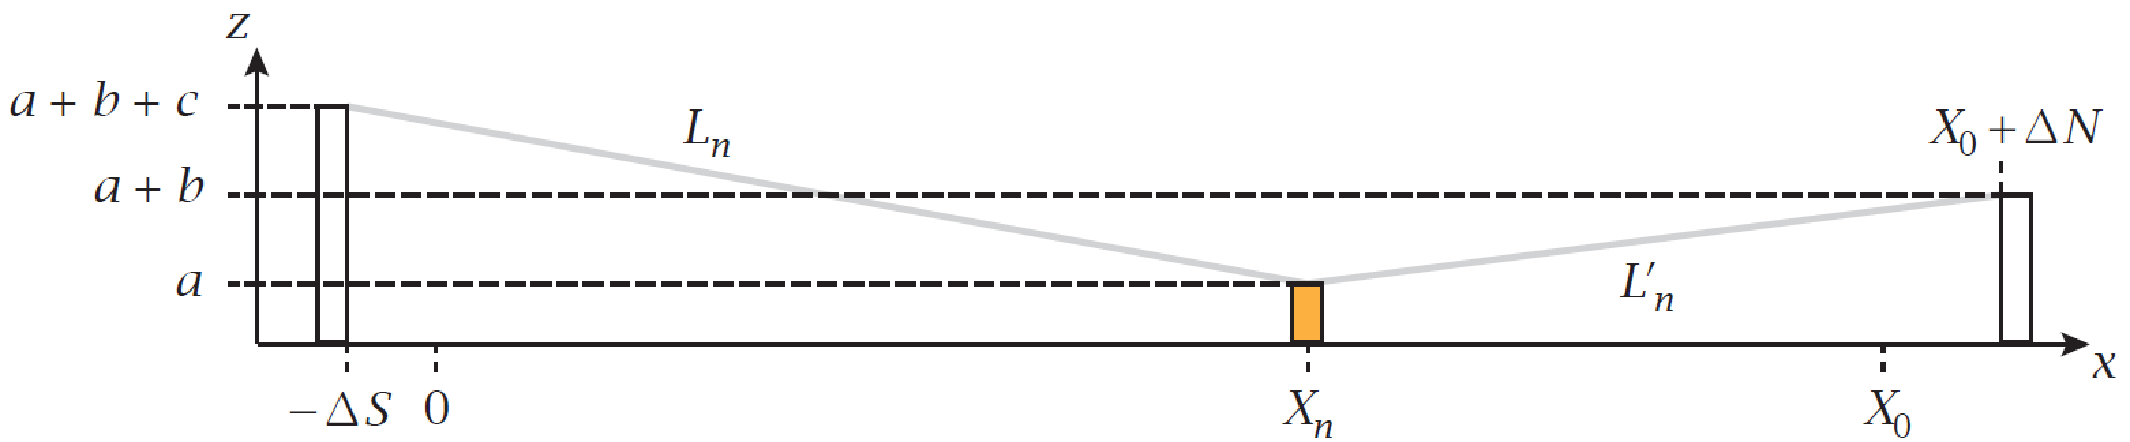
\includegraphics[width=6.0in]{figures/guitar_schematic}
  \caption{\label{fig:guitar_schematic} A simple (side-view) schematic of the classical guitar used in this model. The scale length of the guitar is $X_0$, but we allow the edges of both the saddle and the nut to be set back an additional distance $\Delta S$ and $\Delta N$, respectively. The location on the $x$-axis of the center of the $n^\textrm{th}$ fret is $X_n$. (Note that the $x$-axis is directed toward the left in this figure.) In the $y$ direction, $y = 0$ is taken as the surface of the fingerboard; therefore the height of each fret above the fingerboard is $a$, the height of the nut is $a + b$, and the height of the saddle is $a + b + c$. $L_n$ is the \emph{resonant length} of the string from the saddle to the center of fret $n$, and $L^\prime_n$ is the length of the string from the fret to the nut.}
 \end{figure}

Our model is based on the schematic of the guitar shown in \fig{guitar_schematic}. The scale length of the guitar is $X_0$, but we allow the edges of both the saddle and the nut to be set back an additional distance $\Delta S$ and $\Delta N$, respectively. The location on the $x$-axis of the center of the $n^\textrm{th}$ fret is $X_n$. In the $y$ direction, $y = 0$ is taken as the surface of the fingerboard; the height of each fret is $a$, the height of the nut is $a + b$, and the height of the saddle is $a + b + c$. $L_n$ is the \emph{resonant length} of the string from the saddle to the center of fret $n$, and $L^\prime_n$ is the length of the string from the fret to the nut. The total length of the string is defined as $\mathcal{L}_n \equiv L_n + L^\prime_n$.

Previous studies of guitar intonation and compensation have chosen to include the apparent increase in length of the string caused by both the fretting depth and the shape of the fretted string under the finger~\cite{ref:byers1996cgi,ref:varieschi2010icf}. As the string is initially pressed to the fret, the total length $\mathcal{L}_n$ increases and causes the tension in the string --- which is clamped at the saddle and the nut --- to increase. As the string is pressed further, does the additional deformation of the string increase its tension (throughout the resonant length $L_n$)? There are at least two purely empirical reasons to doubt this hypothesis. First, we can mark a string (with a fine-point felt pen) above a particular fret and then observe the mark with a magnifying glass. As the string is pressed all the way to the finger board, the mark does not move perceptibly --- it has become effectively \emph{clamped} on the fret. Second, we can use either our ears or a simple tool to measure frequencies~\cite{ref:pgtweb} to listen for a shift as we use different fingers and vary the fretted depth of a string. The apparent modulation is far less than would be obtained by classical vibrato ($\pm15$~cents), so we assume that once the string is minimally fretted the length(s) can be regarded as fixed. (If this were not the case, then fretting by different people or with different fingers, at a single string or with a barre, would cause additional, varying frequency shifts that would be audible and difficult to compensate.) We discuss this issue in more detail in \app{fret}.

We start with the form of the fundamental frequency of a fretted string given by \eqn{f_m_stiff} with $m = 1$, and apply it to the frequency of a string pressed just behind the $n^\mathrm{th}$ fret:
 \begin{equation} \label{eqn:f_n_def}
f_n = \frac{1}{2\, L_n}\, \sqrt{\frac{T_n}{\mu_n}} \left[ 1 + B_n + \left(1 + \frac{\pi^2}{2}\right) B_n^2 \right]\, ,
 \end{equation}
where $T_n$ and $\mu_n$ are the modified tension and the linear mass density of the fretted string, and
 \begin{equation} \label{eqn:b_n_def}
B_n \equiv \sqrt{\frac{\pi\, \rho^4\, E}{4\, T_n\, L_n^2}}\, .
 \end{equation}
We note that $T_n$ and $\mu_n$ depend on $\mathcal{L}_n$, the \emph{total} length of the fretted string from the saddle to the nut. Ideally, in the 12-TET system~\cite{ref:durfee2015pms},
 \begin{equation} \label{eqn:f_n_tet}
f_n = \gamma_n\, f_0\, , \qquad \textrm{(12-TET~ideal)}
 \end{equation}
where $f_0$ is the frequency of the open (unfretted) string, and
 \begin{equation} \label{eqn:gamme_n_def}
\gamma_n \equiv 2^{n / 12}\, .
 \end{equation}
Therefore, the error interval --- the difference between the fundamental frequency of the fretted string and the corresponding perfect 12-TET frequency --- expressed in cents is given by
 \begin{equation}\label{eqn:error_def}
 \begin{split}
\Delta \nu_n &= 1200\, \log_2\left( \frac{f_n}{\gamma_n\, f_0} \right) \\
%&= 1200\, \log_2 \left( \frac{L_0}{\gamma_n\, L_n}\, \sqrt{\frac{\mu_0}{\mu_n}\, \frac{T_n}{T_0}}\, \frac{1 + B_n}{1 + B_0} \right) \\
&= 1200\, \log_2 \left( \frac{L_0}{\gamma_n\, L_n} \right) + 600\, \log_2 \left(  \frac{\mu_0}{\mu_n} \right) + 600\, \log_2 \left( \frac{T_n}{T_0} \right) \\
&\qquad + 1200\, \log_2 \left[ \frac{1 + B_n + (1 + \pi^2/2)\, B_n^2}{1 + B_0 + (1 + \pi^2/2)\, B_0^2} \right]\, .
 \end{split}
 \end{equation}

The final form of \eqn{error_def} makes it clear that --- for nylon guitar strings --- there are four contributions to intonation:
 \begin{enumerate}
  \item
   \emph{Resonant Length}: The first term represents the error caused by the increase in the length of the fretted string $L_n$ compared to the ideal length $X_n$, which would be obtained if $b = c = 0$ and $\Delta S = \Delta N = 0$.
  \item
   \emph{Linear Mass Density}: The second term is the error caused by the reduction of the linear mass density of the fretted string. This effect will depend on the \emph{total} length of the string, given by $\mathcal{L}_n = L_n + L^\prime_n$.
  \item
   \emph{Tension}: The third term is the error caused by the \emph{increase} of the tension in the string arising from the stress and strain applied to the string by fretting. This effect will also depend on the total length of the string $\mathcal{L}_n$.
  \item
   \emph{Bending Stiffness}: The fourth and final term is the error caused by the change in the bending stiffness coefficient caused by changing the vibrating length of the string from $L_0$ to $L_n$.
 \end{enumerate}
Note that the properties of the logarithm function have \emph{decoupled} these physical effects by converting multiplication into addition. We will discuss each of these sources of error in turn below.

 \subsection{Resonant Length}
We can estimate the first term in the last line of \eqn{error_def} by referring to \fig{guitar_schematic} and computing the resonant length $L_n$. We find:
 \begin{equation}  \label{eqn:l_n_def}
L_n = \begin{cases}
\sqrt{\left(X_0 + \Delta S + \Delta N\right)^2 + c^2} & n =  0\, , \\
\sqrt{\left(X_n + \Delta S\right)^2 + (b + c)^2} & n \ge 1\, .
 \end{cases}
 \end{equation}
When $b + c \ll X_0$, we can use a Taylor series to approximate $L_n$ by
 \begin{equation} \label{eqn:l_n_approx}
L_n \approx \begin{cases}
X_0 + \Delta S + \Delta N + c^2/2\, X_0 & n =  0\, , \\
X_n + \Delta S + (b + c)^2/2\, X_n & n \ge 1\, .
 \end{cases}
 \end{equation}
Then --- when the guitar has been manufactured such that $X_n = X_0 / \gamma_n$ --- the resonant length error is approximately
%  \begin{equation}
%  1200\, \log_2 \left( \frac{L_0}{\gamma_n\, L_n} \right) \approx -\frac{1200}{\ln(2)} \left[ \frac{\left(\gamma_n - 1\right) \Delta S - \Delta N}{X_0} + \frac{\gamma_n^2 (b + c)^2 - c^2}{2\, X_0^2}\right]
%  \end{equation}
  \begin{equation} \label{eqn:rle_approx}
  1200\, \log_2 \left( \frac{L_0}{\gamma_n\, L_n} \right) \approx \frac{1200}{\ln(2)} \left[ \frac{\Delta N - \left(\gamma_n - 1\right) \Delta S}{X_0} - \frac{\gamma_n^2 (b + c)^2 - c^2}{2\, X_0^2}\right]
  \end{equation}
If the guitar is uncompensated, so that $\Delta S = \Delta N = 0$, this error is typically less than 0.25~cents. But, with $\Delta S > 0$ and $\Delta N < 0$, we can significantly \emph{increase} the magnitude of this ``error'' and cause the frequency to shift lower. We'll see that this is our primary method of compensation.

 \subsection{Linear Mass Density}
As discussed above, the linear mass density $\mu_0$ of an open (unfretted) string is simply the total mass $M$ of the string clamped between the saddle and the nut divided by the length $L_0$. Similarly, the mass density $\mu_n$ of a string held onto fret $N$ is $M/\mathcal{L}_n$. Therefore
 \begin{equation}
\frac{\mu_0}{\mu_n} = \frac{\mathcal{L}_n}{L_0} \equiv 1 + Q_n\, ,
 \end{equation}
where we have followed Byers and defined~\cite{ref:byers1996cgi,ref:varieschi2010icf}
 \begin{equation} \label{eqn:q_n_def}
Q_n \equiv \frac{\mathcal{L}_n - L_0}{L_0}\, .
 \end{equation}
Since we expect that $Q_n \ll 1$, we can approximate the second term in the final line of \eqn{error_def} as
 \begin{equation} \label{eqn:lmd_error}
600\, \log_2 \left(  \frac{\mu_0}{\mu_n} \right) \approx \frac{600}{\ln(2)}\, Q_n\, .
 \end{equation}

Referring to \fig{guitar_schematic}, we see that $\mathcal{L}_n = L_n + L^\prime_n$, and we calculate $L^\prime_n$ for $n \ge 1$ as
 \begin{equation} \label{eqn:l_p_def}
L^\prime_n = \sqrt{\left(X_0 - X_n + \Delta N\right)^2 + b^2} \approx X_0 - X_n + \Delta N + \frac{b^2}{2 \left(X_0 - X_n\right)}\, ,
 \end{equation}
where the approximation applies when $b^2 \ll X_0 - X_n$. Therefore, using \eqn{l_n_approx}, we have
 \begin{equation}
\mathcal{L}_n = L_n + L^\prime_n \approx X_0 + \Delta S + \Delta N + \frac{(b + c)^2}{2\, X_n} + \frac{b^2}{2 \left(X_0 - X_n\right)}\, ,
 \end{equation}
and
 \begin{equation} \label{eqn:q_n_approx}
 \begin{split}
Q_n &\approx \frac{1}{2\, X_0} \left[ \frac{(b + c)^2}{X_n} + \frac{b^2}{X_0 - X_n} - \frac{c^2}{X_0} \right] \\
&= \frac{\gamma_n}{2\, X_0^2} \left[ (b + c)^2 + \frac{b^2}{\gamma_{n} - 1} - \frac{c^2}{\gamma_n} \right] \, .
 \end{split}
 \end{equation}
In \fig{qn_test}, we plot a comparison between the exact expression for the normalized displacement $Q_n$ given by \eqn{q_n_def} with the approximate expression given by \eqn{q_n_approx}. Here the guitar has $b = 1.0$~mm, $c = 3.5$~mm, $\Delta S = 1.5$~mm, $\Delta N = -0.25$~mm, and $X_0 = 650$~mm. We see that our Taylor series estimate is quite accurate even though it neglects both setbacks, indicating that $Q_n$ is determined primarily by the values of $b$ and $c$. For the same parameters, $\Delta \nu_{12} \approx 0.03$~cents, and will be even smaller for $n < 12$. In general, the shift due to linear mass density can be neglected without much loss of accuracy.

%If we add this shift due to the linear mass density to the residual quadratic resonant length shift given by \eqn{rle_approx}, then we find the total error
% \begin{equation} \label{eqn:quad_shift}
%\Delta \nu_n = \frac{300}{\ln(2)}\, \frac{\gamma_n}{X_0^2} \left[ \frac{b^2}{\gamma_n - 1} + \frac{c^2}{\gamma_n} - (2 \gamma_n - 1) (b + c)^2 \right]\, .
% \end{equation}
%For the same parameters, $\Delta \nu_{12} = -0.11$~cents, and $|\Delta \nu_n| < |\Delta \nu_{12}|$ for $n < 12$.

 \begin{figure}
  \centering
  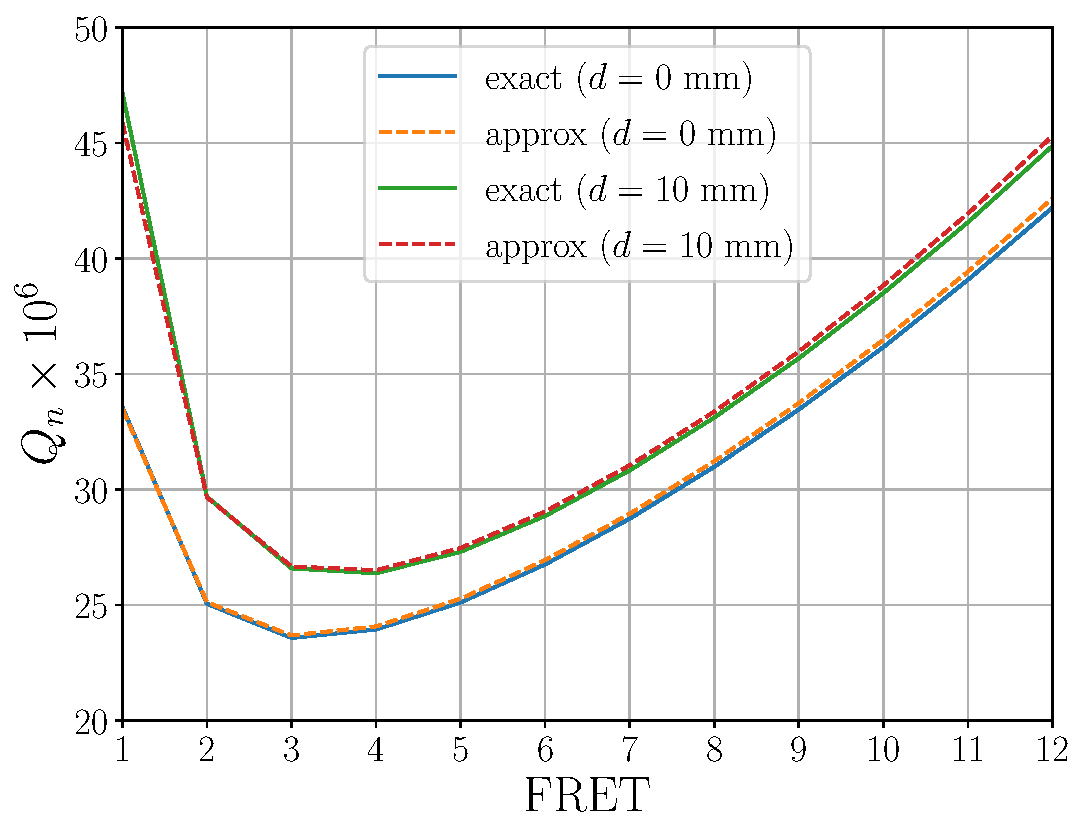
\includegraphics[width=6.0in]{figures/qn_test}
  \caption{\label{fig:qn_test} Comparison of the exact expression for the normalized displacement $Q_n$ as a function of the fret number given by \eqn{q_n_def} with the approximate expression given by \eqn{q_n_approx}. Here the guitar has $b = 1.0$~mm, $c = 3.5$~mm, $\Delta S = 1.5$~mm, $\Delta N = -0.25$~mm, and a scale length of 650~mm.}
 \end{figure}


 \subsection{Tension\label{sct:model_tension}}
%The third term in \eqn{error_def} provides us withe frequency shift of a string
Elasticity properties~\cite{ref:landau1986toe}
 \begin{equation} \label{eqn:youngs_mod_def}
\Delta T_n = E\, A\, \frac{\mathcal{L}_n - L_0}{L_0} = A\, E\, Q_n\, ,
 \end{equation}
where we have used \eqn{q_n_def}. Therefore, the tension of the fretted string is
 \begin{equation}
T_n = T_0 + \Delta T_n = T_0 \left( 1 + \kappa\, Q_n \right)\, ,
 \end{equation}
where we have defined the dimensionless ``string constant''
 \begin{equation}\label{eqn:kappa_def}
\kappa \equiv \frac{A\, E}{T_0} = \frac{\pi \rho^2 E}{T_0}\, .
 \end{equation}
In this case, we assume that $\kappa Q_n \ll 1$, so that we can approximate the third term in the final line of \eqn{error_def} as
 \begin{equation}
600\, \log_2 \left(  \frac{T_n}{T_0} \right) \approx \frac{600}{\ln(2)}\, \kappa\, Q_n\, .
 \end{equation}
This frequency shift is larger than that caused by the linear mass density error by a factor of $\kappa$.

 \subsection{Bending Stiffness}
% \begin{equation}
%f_{m n} = \frac{m}{2\, L_n}\, \sqrt{\frac{T_n}{\mu_n}} \left( 1 + B_n \right)\, ,
% \end{equation}

Since $B_n$ is already relatively small, we only need to consider the largest contribution arising from the shortened length of the fretted string compared to that of the open string. We see from \eqn{l_n_def} that $L_n \approx L_0/\gamma_n$, so from \eqn{b_n_def} we have
 \begin{equation}
B_n = \sqrt{\frac{\pi\, \rho^4\, E}{4\, T_n\, L_n^2}} \approx \frac{L_0}{L_n}\, \sqrt{\frac{\pi\, \rho^4\, E}{4\, T_0\, L_0^2}} = \gamma_n\, B_0\, .
 \end{equation}
Therefore, the fourth term in the final line of \eqn{error_def} can be approximated as
 \begin{equation}
1200\, \log_2 \left[ \frac{1 + B_n + (1 + \pi^2/2)\, B_n^2}{1 + B_0 + (1 + \pi^2/2)\, B_0^2} \right] \approx \frac{1200}{\ln(2)}\, \left[ \left(\gamma_n - 1\right) B_0 + \half\, \left(\gamma_n^2 - 1\right) \left(1 + \pi^2\right) B_0^2 \right]\, .
 \end{equation}
When $n = 12$ and $B_0 = 6 \times 10^{-3}$, the corresponding shift is approximately 5.5~cents, with the quadratic term contributing about 0.25~cents. Note that (to zero order in $Q_n$) this bending stiffness error does not depend on the tiny changes to the linear mass density or the tension that arises due to string fretting. Instead, it is an intrinsic property of the string.\bigskip

Incorporating all of these effects --- and neglecting the term proportional to $B_0^2$ --- we find that the total frequency shift is given by
 \begin{equation}\label{eqn:error_tot}
\Delta \nu_n \approx \frac{1200}{\ln(2)}\, \left[ \left(\gamma_n - 1\right) \left(B_0 - \frac{\Delta S}{X_0}\right) + \frac{\Delta N}{X_0} + \half\, \kappa\, Q_n \right]\, .
 \end{equation}
In this form, we see that the bending stiffness and the increase in string tension due to fretting sharpen the pitch, but that we can flatten it with a positive saddle setback and negative nut setback. In fact, a simple compensation strategy would be to choose $\Delta S = B_0\, X_0$ to compensate for stiffness, and then select $\Delta N = - \kappa\, X_0\, \overline{Q} / 2$, where $\overline{Q}$ is the displacement averaged over a particular set of frets. We'll choose a more flexible method for compensation in \sct{comp}, but we'll obtain results that are similar to this basic approach. 